%!TEX root = ../main.tex

\chapter{Introduction}
\markboth{Introduction}{}
%\vspace{-1.3in}



\section{Embedded Systems}

An embedded system constitutes a specialized computing system engineered to execute predetermined application-specific tasks, contrasting with the versatility of general-purpose computers. Its defining attributes encompass the inclusion of at least one microcontroller, compact physical dimensions, low cost, and adherence to strict resource limitations. It is crucial to emphasize that the primary differentiation between an embedded system and a conventional computer stems not from their size but from their designated functionalities. The complexity of embedded systems can vary, ranging from rudimentary configurations with minimal peripherals to intricate systems present in airplanes.

At the core of an embedded system lies at least one microprocessor or microcontroller programmed to run a specific software application. This process of "specialization" in embedded systems enables their designers to optimize these systems, yielding enhancements in size, cost-efficiency, execution speed, or power efficiency.  Predominant architectures prevalent in embedded systems are ARM, MIPS, PowerPC, Microblaze, and X86.




\section{FPGA's}
FPGA (Field Programmable Gate Array) is a type of general-purpose programmable integrated circuit that features a multitude of logic components such as Look-up Tables (LuTs), logic gates, counters, memory registers, PLL generators, and sometimes it can also include analog functions. The basic unit of an FPGA is the Logic Block (LB) which is a predetermined collection of such basic components. Additionally, there are blocks responsible solely for the input/output of the FPGA (I/O Blocks). LBs and IO Blocks are interconnected either with fixed wiring or through switch matrices.

In the process of FPGA programming, specific logic elements are configured to perform a specific function,  while the requisite interconnections are activated to facilitate the desired data flows.  After programming, the FPGA operates akin to a custom-integrated circuit built to execute the programmed functionality.

In the case of Xilinx FPGAs, LBs are called Configurable Logic Blocks (CLBs) and are partitioned into smaller units called slices. The configuration and composition of CLBs and slices vary across FPGA families. Depending on the specific FPGA variant, a CLB may accommodate 2, 4, or 6 slices.
Each slice comprises LUTs and possibly predefined logic components, such as small multiplexers, logic gates, and adders. Depending on the FPGA family, LuTs may be (4 inputs/1 output) or (6 inputs/2 outputs). The composition of predefined logic components also varies, from generic logic gates to  Digital Signal Processing (DSP) components. An example CLB is shown in Figure ~\ref{fig:figure_1.1}.


\begin{figure}
\centering
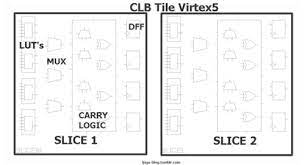
\includegraphics[width= 0.4\textwidth]{figure_1.1}\\
\caption{Structure of a Xilinx Virtex-5 Configurable Logic Block (CLB)}
\label{fig:figure_1.1}
\end{figure}

FPGAs are available either as standalone chips suitable for integration onto printed circuit boards (PCBs) or as part of integrated solutions where the FPGA is embedded within a specialized board. These integrated solutions typically come equipped with a module responsible for the FPGA programming and offer a range of standard interfaces including serial ports (UART), and Ethernet, as well as interfaces for external memory and storage devices.

\pagebreak
The primary advantages of FPGAs over traditional implementations include:
\begin{outline}
\1 FPGAs occupy a strategic middle ground between software-based solutions and Application-Specific Integrated Circuits (ASICs), offering faster implementations compared to software-based approaches, while remaining more cost-effective than ASICs.

\1 FPGAs liberate designers from reliance on component manufacturing and distribution chains, as the behavior of the device is not inherent to its physical structure but is determined by the designer's configuration.

\1 The reprogrammable nature of FPGAs fosters reusability and facilitates upgradability, enabling iterative refinement of designs without necessitating hardware replacements.

\end{outline}

\section{Communication Networks}
A computer network is defined as a set of interconnected devices purposed for facilitating communication among them.  Different types of networks exist, depending on their intended functions and operational constraints. The Internet is the largest network of interconnected computing devices.

Various technologies are available to choose from when connecting devices, including Ethernet cables, optical fibers, and wireless mediums leveraging electromagnetic waves such as microwaves. The selection of a particular technology depends on several criteria, with the most important considerations being performance and cost-effectiveness.

In addition to establishing physical interconnectivity among systems, the formulation of precise rules and communication protocols is required for any communication attempts to be successful. These communication protocols serve as the foundational framework underpinning the proliferation and diversification of network-centric applications.

Another important characteristic of networks is the transmission of information in the form of packets. Each packet encapsulates either the entirety or a portion of the transmitted data. Alongside the information intended to be transmitted (payload), packets include one or more headers containing information needed for the transmission of the packet itself. Intermediate network nodes leverage this header information to facilitate packet routing, whereas the payload content is exclusively intended for consumption by the ultimate recipient.


\subsection{Protocol Stack}
% Networks are based on the principle of modularity, meaning their entire operation is divided into individual and, as much as possible, independent functions. This approach allows us to address the complexity of these systems and, furthermore, makes them more flexible, as any necessary changes can be made without needing to rework the entire implementation, but only the relevant part.

Networks are structured upon the foundational principle of modularity, wherein their operational framework is compartmentalized into discrete and ideally autonomous functions. This modular approach not only reduces the inherent complexity of these systems but also enables flexibility and adaptability since modifications don't require a comprehensive overhaul of the entire architecture but rather focus on relevant segments.

% The protocol stack is a series of layers or levels of information processing for transmission/reception. This processing aims at the successful transmission/reception of information from one system (host) to another, and for successful communication, the stack must be implemented at each end of the communication. Each layer undertakes a specific function and provides services to the immediately higher layer of the stack. When information is sent, processing begins from the highest level to the lowest, with the final function being the transmission of data, while during reception, the reverse path is followed until the information is received.

Central to network operation is the protocol stack, comprising a hierarchical arrangement of layers dedicated to information processing of the transmitted information. This processing aims to ensure a seamless exchange of information between systems (hosts). This requires the existence of an implementation of the protocol stack at each end of the communication. Each layer within the stack assumes a distinct function and provides services to the layer above. During the transmission phase, information processing commences from the highest layer and cascades downward, reaching the lower layer where the physical transmission takes place, whereas, in the reception phase, the reverse path is followed, with the upper layer providing the information to the host application.

\begin{figure}
\centering
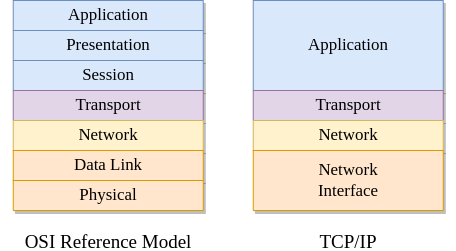
\includegraphics[width= 0.5\textwidth]{figure_1.2}\\
\caption{(left) The OSI stack, (right) the TCP/IP stack}
\label{fig:figure1.2}
\end{figure}

% The structure of the protocol stack has been standardized by the OSI (Open Systems Interconnection) model. The OSI model is based on a proposal developed by the International Standards Organization (ISO) as a first step towards the international standardization of protocols used in various network layers. It abstractly defines the layers, their functions, and their interconnections. It does not specify the protocols used at each layer but simply describes the functions that should be performed at each layer. Thus, there are many different protocols for each layer, each used for different purposes and covering different needs. These layers and their basic functions are:

The protocol stack's architecture is standardized by the OSI (Open Systems Interconnection) model, originating from a proposal developed by the International Standards Organization (ISO) to initiate global standardization of network protocols across diverse layers. The OSI model abstractly delineates these layers, their functionalities, and their interconnections. It refrains from specifying protocols but instead outlines the functions at each layer should perform. Consequently, a multitude of protocols exists for each layer, tailored to distinct purposes and addressing diverse requirements. The OSI layers are outlined as follows:

\begin{outline}
\1 Physical Layer\\
Responsible for data transmission across the physical communication channel, the Physical Layer is tasked with encoding/decoding data into the channel's respective code, such as electrical pulses (e.g., 0-5V for cable transmission) or optical pulses (for optical fiber transmission). Its primary objective is to ensure accurate reception of transmitted bits without degradation or misinterpretation.

\1 Data Link Layer\\
Assuming control over data transmission from the Physical Layer, the Data Link Layer ensures reliable data delivery, encompassing error detection, correction, and recovery procedures. It segments data into discrete frames for transmission and conducts error checking upon reception of each frame. Additionally, it may include traffic regulation mechanisms to regulate data flow and prevent congestion.

\1 Network Layer\\
It orchestrates the routing of information through intermediate systems to facilitate communication between non-directly connected systems and hosts belonging to disparate local networks.

\1 Transport Layer\\
Catering to scenarios where multiple applications or users seek access to the network, the Transport Layer manages the multiplexing and demultiplexing of data, ensuring accurate delivery to the intended recipient(s).

\1 Session Layer\\
Enabling users from different systems to establish sessions, the Session Layer offers services such as dialogue control, token management, and synchronization.

\1 Presentation Layer\\
In contrast to lower layers that focus on bit transmission, the Presentation Layer concerns itself with the syntax and semantics of transmitted information. It manages abstract data structures to facilitate interoperability among systems employing different data representations, facilitating standardized encoding for data exchange

\1 Application Layer\\
Comprising a suite of protocols catering to diverse user requirements, the Application Layer facilitates functions such as file transfer, email communication, and web page presentation. This is the layer where data is created and where transmitted data gets received.
\end{outline}\\


The Internet utilizes the TCP/IP stack, incorporating the TCP (Transmission Control Protocol) and IP (Internet Protocol) as its primary protocols. While adhering to the OSI model, the TCP/IP stack merges the transport and session layers within the application layer. Additionally, the lower layers (physical and data link) are often merged as well, forming a cohesive network interface layer. Figure ~\ref{fig:figure1.2} illustrates the OSI and TCP/IP stacks, highlighting their similarities and differences.

\begin{figure}[h!]
\centering
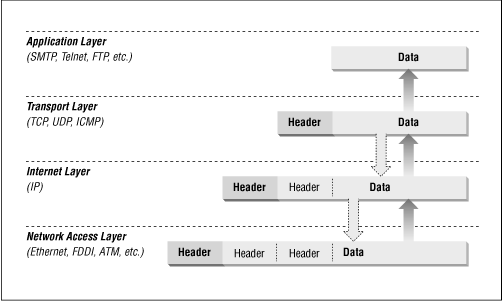
\includegraphics[width= 0.7\textwidth]{figure_1.3}\\
\caption{Packet transformation through the protocol stack}
\label{fig:figure1.3}
\end{figure}


During transmission, data originates at the application layer and traverses sequentially through the protocol stack until it reaches the physical layer for transmission. At each layer, the data received from the layer above is augmented with a suitable header, and in some cases, additional data may be appended to the "tail" of the packet. This iterative process, known as encapsulation, ensures that each layer includes information needed by its corresponding layer on the other side of the communication. During reception, the data first reaches the physical layer and moves upwards in the stack. Each layer successively processes and strips away its corresponding header, thereby progressively unveiling the core content of the packet. The core content is ultimately delivered to the application layer without any headers. The abstract representation of the packet format at each layer is depicted in Figure ~\ref{fig:figure1.3}.

\subsection{Network Security}
% The field of network security deals with the secure communication between networked systems, controlling access to network services and resources, as well as protecting and ensuring the proper functioning of individual systems and the network as a whole. It belongs to the domain of information security and applies basic concepts such as confidentiality and authentication in the realm of networks.

% A fundamental aspect of network security is the design, analysis, and implementation of security protocols. Beginning with the design phase, the objectives and services that the protocol will provide are initially defined. Subsequently, the protocol details are specified, including packet header formats, request-response mechanisms, algorithm usage, and other protocols. Additionally, during the design phase, scenarios under which the protocol will operate are defined and examined.

% Next, we proceed to the analysis phase, where the extent to which the design meets the objectives is evaluated, potential errors or omissions are identified, etc. Analysis may reveal the need for changes or expansions to the protocol design, prompting a redesign. This feedback loop continues until satisfactory results are achieved.

% Following the analysis, comes the implementation of the protocol, which involves considerations of performance, selection of implementation methods (hardware or software, programming language, etc.), and verification. At this stage, particular attention must be paid to the secure implementation of the protocol. Secure implementation does not solely concern the security of the protocol itself but also involves avoiding technical errors that may create security vulnerabilities. Thus, a protocol may offer a significant degree of security, but its implementation may render the system vulnerable to other types of attacks beyond those it was designed to protect against. Secure programming, secure hardware implementation, as well as physical placement and access methods of the system, are all aspects of secure implementation.

% Cryptology plays a significant role in network security as it provides the fundamental tools and mechanisms. Therefore, the security of networks, and information security in general, depends on the security of the cryptographic algorithms used and whether they are employed correctly.

% Common objectives in network security include the confidentiality and integrity of data, certification, availability of resources and services, as well as prevention methods and scenarios for recovering from attacks or malfunctions, concepts that will be elaborated upon in a subsequent chapter.

The domain of network security encompasses the establishment of secure communication channels among networked systems, the regulation of access to network services and resources, and the safeguarding of individual systems and the network as a cohesive entity. As part of the broader context of information security, network security is grounded in fundamental concepts such as confidentiality and authentication, tailored specifically to the realm of network environments.

Central to network security is the design, analysis, and deployment of security protocols. In the design phase, the objectives and services the protocol needs to provide are defined. Subsequently, the protocol details are specified, including packet header formats, request-response mechanisms, and algorithm choices. Furthermore, during the design phase, different operational scenarios are delineated and scrutinized.

In the analysis phase, the efficacy of the design in meeting predefined objectives is rigorously assessed, while potential flaws or oversights are identified and mitigated. The analysis is an iterative refinement process of revisions and enhancements until the protocol design satisfies its objectives.

Following analysis, the protocol is implemented. In this stage implementation and verification methodologies are selected. Of paramount importance is the secure implementation of the protocol. 
Secure implementation involves addressing technical flaws that could unintentionally create security weaknesses. Even if a protocol provides strong security features, an improperly implemented version could expose the system to unforeseen risks. Secure programming practices, secure hardware design, and defining access control are part of the secure implementation phase. The protocol implementation phase also includes performance and reliability considerations.

Cryptography assumes a pivotal role in the realm of network security, providing foundational tools and mechanisms for safeguarding network communications. Network security, and by extension, information security as a whole, relies on the robustness and correct usage of cryptographic algorithms.

Notable objectives of network security include data confidentiality and integrity, attestation mechanisms, resource availability, and the formulation of contingency plans for incident response and recovery, concepts that will be elaborated upon in subsequent chapters.